\documentclass[12pt]{article} 
\usepackage{amsmath} 
\usepackage[english,russian]{babel} 
\usepackage{indentfirst} 
\usepackage{amssymb} 
\usepackage{amsfonts} 
\usepackage{amsthm} 
\usepackage[dvipsnames]{xcolor}
\usepackage{hyperref}
\usepackage[T2A]{fontenc} 
\usepackage[utf8]{inputenc} 
\usepackage{epigraph} 
\usepackage{tikz} 
\usepackage{wrapfig}
\usepackage[noend]{algorithmic} 
\textheight=24cm % высота текста 
\textwidth=16cm % ширина текста 
\oddsidemargin=0pt % отступ от левого края 
\topmargin=-1.0cm % отступ от верхнего края 
\parindent=24pt % абзацный отступ 
\parskip=0pt % интервал между абзацами 
\tolerance=2000 % терпимость к "жидким" строкам 
\flushbottom % выравнивание высоты страниц %
\def\baselinestretch{1.5} % печать с большим интервалом
\usepackage{tikz}

\begin{document}

%% выключаем отображение номера для этой страницы (титульник)
\thispagestyle{empty}

\newpage
\begin{center}
\textbf{\large МОСКОВСКИЙ ФИЗИКО-ТЕХНИЧЕСКИЙ ИНСТИТУТ\\ (НАЦИОНАЛЬНЫЙ ИССЛЕДОВАТЕЛЬСКИЙ УНИВЕРСИТЕТ)}

\vspace{0.5cm}

Физтех-школа прикладной математики и информатики

Кафедра банковских информационных технологий

\vspace{0.5cm}


\includegraphics[width=7cm]{images/emblema.jpg}

\vspace{0.5cm}

\textbf{\Large Сравнение трансформера и градиентного бустинга в задаче кредитного скоринга}
\end{center}

\vspace{2cm}


\begin{flushright}
    \textbf{Автор:} \\
    Студент группы Б05-103 \\
    Царев Иван Николаевич \\
    \vspace{2em}
    \textbf{Научный руководитель:} \\
    Филлипенков Николай Владимирович \\
\end{flushright}

\vfill

\begin{center}
Москва, 2025 г.
\end{center}

\newpage
\section*{Аннотация}

В рамках данного исследования рассматриваются современные подходы к решению задачи кредитного скоринга. Цель данной работы - сравнение передовых архитектур нейронных сетей, преимущественно основанных на применении трансформерных слоев, и методов классического машинного обучения, а именно, градиентного бустинга в задаче кредитного скоринга.

В ходе работы были спроектированы и реализованы несколько архитектур нейронных сетей, адаптированных для работы с табличными данными. Кроме того, реализовано несколько методов предварительной обработки данных - эмбедингов, которые оказывают существенное влияние на качество модели. Все полученные модели были протестированы на нескольких публичных датасетах и сравнены с реализацией градиентного бустинга из библиотеки \texttt{CatBoost}, которая в настоящее время считается одной из самых эффективных.

Основным результатом работы является демонстрация того, что нейронные сети способны эффективно работать в задаче кредитного скоринга и обеспечивать качество предсказаний, сопоставимое с современными реализациями градиентного бустинга. Более того, при правильной настройке нейронных сетей возможно достижение более высоких результатов. Представленный подход показывает потенциал использования нейронных сетей даже в таких специфических задачах, как кредитный скоринг, и может стимулировать дальнейшие исследования в области применения глубокого обучения к табличным данным.


\onehalfspacing
\setcounter{page}{2}

\newpage
\addcontentsline{toc}{section}{Содержание}
\tableofcontents

\newpage

\section{Введение}

\subsection{Кредитный скоринг}

Кредитный скоринг играет ключевую роль в современном финансовом мире. Скоринг - процесс, результатом которого, является оценка кредитоспособность клиента (обычно на выходе ожидается вероятность дефолта клиента). Современные скоринговые модели учитывают множество поведенческих признаков пользователя, таких как кредитная история, финансовое положение, личные данные и даже история его покупок на маркетплейсах, поездок на такси и заказов в сервисах доставки еды. Важно понимать, что кредитный скоринг помогает банкам минимизировать риски, связанные с невозвратом кредитов, обеспечивая их более эффективную выдачу.

Актуальность задачи кредитного скоринга в наши дни сложно переоценить. В условиях быстро меняющейся экономической ситуации точные модели кредитного скоринга становятся жизненно необходимыми для крупных компаний. Скоринг используется посвюду: в банках, микрофинансовых организациях (МФО), BNPL-сервисах (\textit{Buy Now, Pay Later}) и страховых фирмах.

Для бизнеса кредитный скоринг – это способ снижения финансовых рисков и оптимизации внутренних процессов. Благодаря автоматизации этого процесса и внедрению современных технологий машинного обучения, компании могут сократить время обработки заявок до нескольких миллисекунд. 

Успешное управление кредитными рисками способствует увеличению прибыли и укреплению финансовых показателей. Например, в крупнейших банках России процентные доходы составляют значительную долю от прибыли: Т-Банк\footnote{\href{https://journal.tinkoff.ru/news/review-bank-industry-2023/}{Источник: журнал Тинькофф, 2023}} в своем отчете за 2023 год показал, что $37\%$ от всей прибыли банка это процентные доходы.

С другой стороны, качественный кредитный скоринг влияет на повседневную жизнь граждан,  обеспечивая им более легкий доступ к финансовым ресурсам. Люди могут быстрее получать кредиты на крупные покупки, такие как техника, недвижимость или автомобиль.

\newpage
\subsection{История решения задачи кредитного скоринга}

Кредитный скоринг прошел долгий путь развития от ручных правил до современных сложных и автоматизированных систем. 

В первых скоринговых системах решения принимались кредитными экспертами вручную, основываясь на их опыте и субъективном мнении. Этот процесс был не только трудоемким, но и подверженным человеческим факторам, что ограничивало его масштабируемость, точность и непредвзятость.

Повышение спроса на кредитные услуги, особенно с введением кредитных карт, подчеркнуло необходимость автоматизации принятия решений. В 1941 году Давид Дюран представил первую исследовательскую работу по кредитному скорингу, где он оценивал значимость различных факторов. Это положило начало развитию более структурированной методологии в этой области.

Ключевой вехой стало появление в 1956 году компании FICO, которая начала активно разрабатывать автоматизированные системы для оценки кредитоспособности. В 1960-х годах началось внедрение компьютерных технологий для обработки больших объемов данных, что существенно повысило эффективность скоринга.

Логистическая регрессия сделала возможной более точную и объективную оценку, позволяя обрабатывать множество параметров в автоматическом режиме. Однако на этом технологический прогресс не остановился: в начале 2000-ых появились более сложные методы, такие как ансамбли деревьев решений, в частности методы градиентного бустинга.

Сейчас же на пороге стоят нейронные сети, которые превосходят классические ML-алгоритмы в эффективности во многих сферах. Задача кредитного скоринга приносит огромную прибыль крупнейшим корпорациям мира, делая ее решение передовой научной областью и предметом конкурентной борьбы за точность.

\newpage
\subsection{Методы решения}

За последние два десятилетия градиентный бустинг стал наверное самым популярным алгоритмом машинного обучения для задач на табличных данных. Он применяется во всех BigTech компаниях для большого числа задач, таких как ранжирование поисковой выдачи, прогнозирование спроса, предсказание оттока пользователей и, конечно, для кредитного скоринга. Популярность градиентного бустинга на деревьях, связана с его высокой эффективностью, простотой и доступностью (есть множество библиотек, в которых GBDT уже реализован).

Нейронные сети, напротив, зарекомендовали себя в областях, требующих обработки сложных и неструктурированных данных: изображений, текстов, звуков и последовательностей. Способность выявлять глубокие нелинейные зависимости сделала их незаменимыми в задачах компьютерного зрения, обработки естественного языка и распознавания речи. В рамках кредитного скоринга также существуют задачи, которые уже давно и успешно решаются нейросетями. Например, многие банки используют различные виды рекуррентных нейронок (\texttt{RNN}) для анализа клиента по истории его транзакций.

Однако при работе с табличными данными - данными хранящимися в виде таблицы, где каждая строка - отдельный объект, а каждый столбец — признак объекта, нейронные сети до сих пор не получили широкого распространения [12]. В этих случаях градиентный бустинг продолжает оставаться самым популярным инструментом благодаря своей эффективности и оптимальному соотношению затрат на обучение и полученного качества.

В последние несколько лет интерес к применению глубокого обучения на табличных данных заметно возрос. Исследователи из таких компаний, как \textit{Yandex}, \textit{Google}, \textit{Amazon} каждый год представляют на конференциях уровня \texttt{NIPS} новые статьи посвященные этой задаче. А работы [1, 2, 5, 6] показывают, что с помощью специальных архитектур нейронных сетей, взятых зачастую совсем из другой задачи (например: из обработки естественного языка или компьютерного зрения), адаптированных к формату табличных данных, можно получить результаты, сопоставимые классическим методам.

Несмотря на потенциал, нейронные сети сталкиваются с рядом сложностей при применении к табличным данным. Их разработка требует тщательного продумывания и написания архитектуры, а обучение - длительное и ресурсоёмкое. Также, для нейронок может быть критически важным наличие большого объёма данных для эффективного обучения, что особенно проблематично для задачи кредитного скоринга, ведь каждый таргет в обучении - потерянные деньги банка. 

Кроме того, выданные кредиты уже проходят какую-то проверку (модельную или ручную), а значит все данные в обучении - смещенные, они характеризуют только часть потока, что может плохо сказаться на разделяющей способности модели. Чтобы избежать такой проблемы, банки обычно запускают шлюз (часть потока, на которой не применяются никакие рисковые правила), чтобы исследовать весь поток целиком. При этом, шлюз обычно очень небольшого размера из-за высокой стоимости.

 Несмотря на это нейронки обладают важными преимуществами над методами классического машинного обучения:
\begin{itemize}
    \item Экономия времени на обработку датасетов: разработчикам не нужно придумывать и генерировать фичи вручную, нейронка работает как черный ящик, на вход которому достаточно подать всю информацию.
    
    \item Упрощенная работа с разнородными признаками: нейронки хорошо работают как с временными рядами (например транзакциями), так и с обычными табличными данными. Бустинг же с последовательными данными работать в принципе не умеет, поэтому их нужно вручную преобразовывать в фичи (например путем агрегации по окнам разной длины).
    
    \item Быстрая адаптация к быстро меняющимся рыночным условиям путем постоянного дообучения существующей модели на новых данных.
\end{itemize}

Новизна темы диплома заключается в исследовании применения различных адаптаций современных нейронных сетей для задачи кредитного скоринга на табличных данных, что сейчас является недоизученным. Традиционные методы, такие как градиентный бустинг, доминируют в этой области, поэтому потенциальное использование нейронных сетей может открыть новые возможности. Это перспективное направление объединяет передовые технологии в сфере глубинного обучения с практическими задачами, представляющими высокий интерес для крупного бизнеса.

\subsection{Постановка задачи и цели работы}

Целью данной работы является проведение сравнительного анализа различных архитектур нейронных сетей и алгоритмов градиентного бустинга на примере задачи бинарной классификации на табличных данных, а именно - задачи кредитного скоринга. 

Основная задача - реализовать адаптированные архитектуры нейронных сетей и провести их оценку на различных банковских датасетах с пользовательскими фичами. Для этого используются открытые данные, такие как датасеты с соревнований на платформе \texttt{Kaggle}, организованных различными крупными банками, например \textit{HomeCreditBank} и \textit{Raiffeisen}.

Для обеспечения объективности и значимости результаты нейронных сетей сравниваются с показателями популярных алгоритмов градиентного бустинга, а именно с \texttt{CatBoost}, который в настоящее время считается одним из лучших алгоритмов для обработки табличных данных и широко применяется в индустрии благодаря своей высокой точности, скорости и простоте использования.

\newpage
\section{Архитектура нейронной сети}

\subsection{Baseline}
Для оценки эффективности продвинутых архитектур нейронных сетей необходимы базовые модели, с которыми можно сравнивать результаты. В качестве таких бейзлайнов, я выбрал две очень простые, но эффективные архитектуры - \texttt{MLP} и \texttt{ResNet}.

\subsubsection{MLP}

Полносвязная нейронная сеть или многослойный перцептрон (MLP) - самая простая архитектура искусственной нейронной сети, в которой каждый нейрон соединен со всеми нейронами следующего слоя.

\vspace{-4mm}
\begin{center}
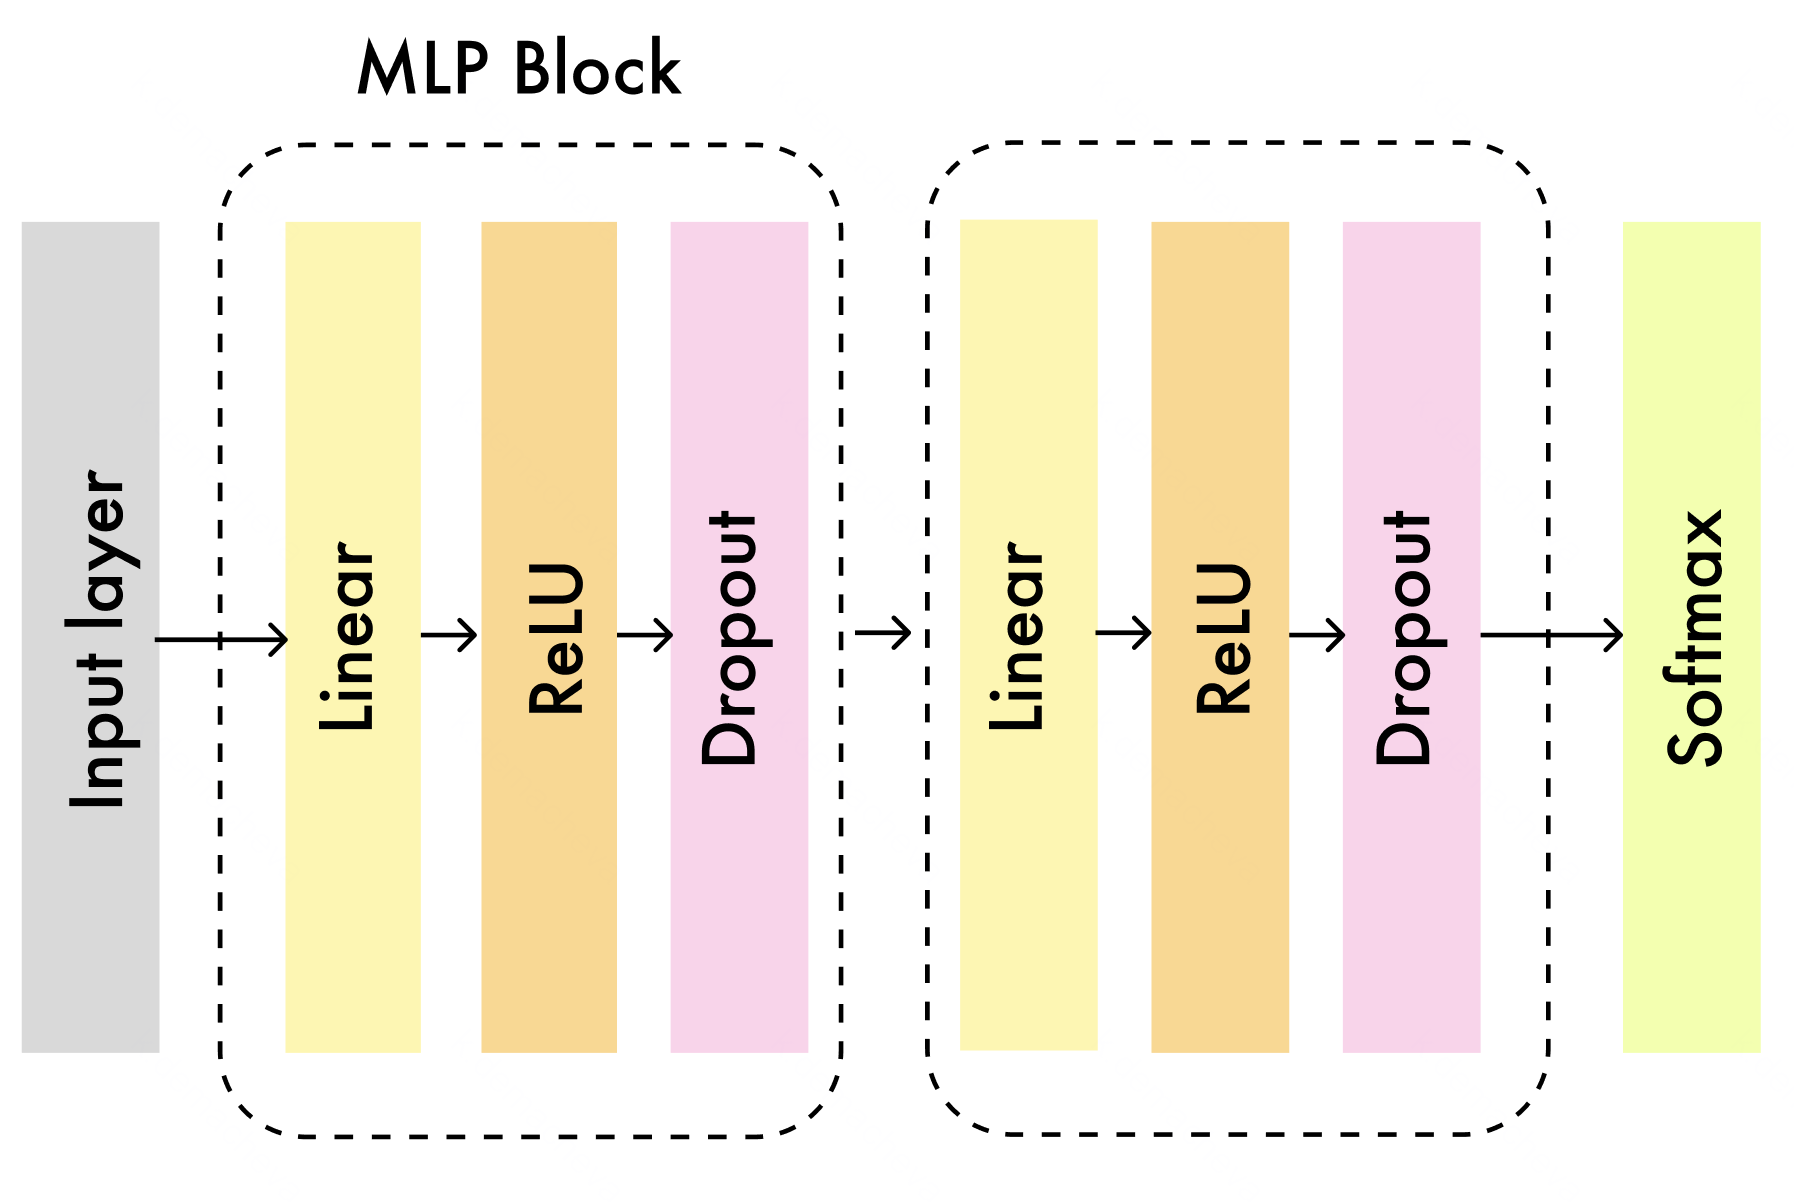
\includegraphics[width=14cm]{images/MLP_v2.png}
\end{center}
\vspace{-5mm}

\noindent MLP состоит из блоков, в каждом из которых выполняются следующие операции:

\begin{enumerate}
    \item Линейное преобразование над входящими данными $x \in \mathbb{R}^d$, с обучаемыми параметрами: матрица весов $W \in \mathbb{R}^{d\times k}$ и вектор смещения $b \in \mathbb{R}^k$
    \begin{equation}
        x \;\mapsto\; xW + b,
    \end{equation}
    
    \item Применение функции активации - нелинейного преобразования, поэлементно применяющееся к пришедшим на вход данным:
    \begin{equation}
        x \;\mapsto\; \sigma(x) = \sigma(xW + b)
    \end{equation}
    где $\sigma(\cdot)$ — какая-то нелинейная функция, например: 
    
    ReLU: $\sigma(x) = \max(0, x)$

    Sigmoid: $\sigma(x) = \frac{1}{1 + \exp^{-x}}$
    
    Кроме того, в архитектуре MLP часто применяется функция активации SELU, которая была предложена в статье \textit{"Self-Normalizing Neural Networks" (2017)} [8]. 
    \begin{equation}
        \mathrm{SELU:} \; \sigma(x) = \lambda 
        \begin{cases} 
        x, & \text{если } x > 0 \\ 
        \alpha e^x - \alpha, & \text{если } x \leq 0 
        \end{cases}
    \end{equation}
    Автор утверждает, что SELU (Scaled Exponential Linear Unit) решает проблемы затухания и взрыва градиентов, ускоряя обучение MLP.

    \item Dropout - метод регуляризации нейронных сетей, который на этапе обучения случайно отключает (зануляет выходы) некоторые нейроны с вероятностью $p$.
\end{enumerate}

\noindent Модель MLP требует относительно небольших вычислительных ресурсов в процессе обучения, поэтому в дальнейшем именно на этой архитектуре проводилось тестирование различных типов эмбедингов.

\subsubsection{ResNet}

Нейронные сети достигли значительных успехов в различных областях, однако по мере увеличения глубины сети возникает проблема затухающих градиентов, что затрудняет обучение глубоких моделей. Поэтому в 2015 году команда под руководством Кайминга Хэ предложила архитектуру Residual Network (ResNet) [10], которая позволила эффективно обучать сети глубиной в сотни слоёв.

Ключевая идея ResNet заключается во введении \textit{skip connections}, которые позволяют сигналу обходить один или несколько слоёв сети. Это означает, что каждый последующий слой учится не непосредственно преобразовывать входные данные, а корректировать или добавлять остаток к выходу предыдущего слоя. Такой подход предотвращает проблемы с затуханием или взрывом градиентов.

Учитывая успешное применение ResNet в компьютерном зрении [10] и его недавние достижения в обработке естественного языка NLP [17], я решил использовать модифицированную архитектуру ResNet в задаче кредитного скоринга. Структурный блок упрощён по сравнению с оригинальной архитектурой: фактически это MLP с добавлением батч нормализации и skip connection.

\begin{flushleft}
    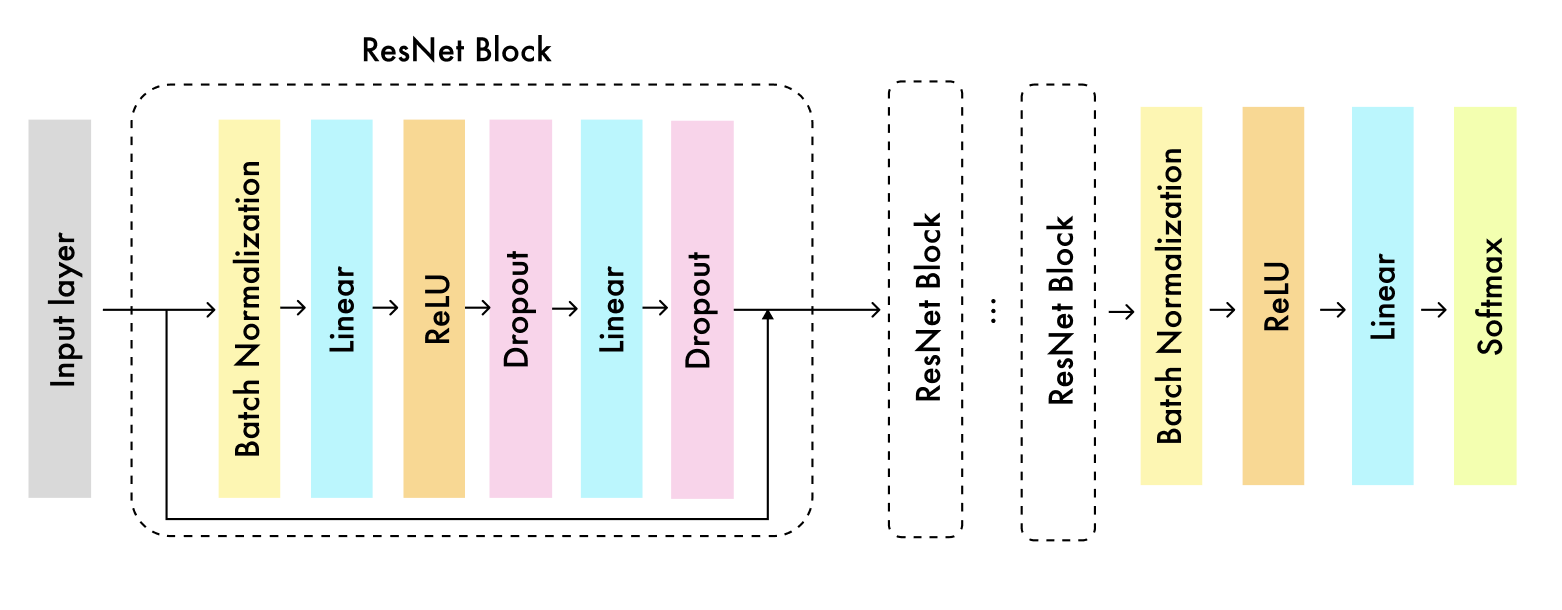
\includegraphics[width=16cm]{images/ResNet_v2.png}
\end{flushleft}


\subsection{Трансформеры}

\subsubsection{Что такое трансформер?}

Как известно, почти все значимые достижения последних лет в области машинного обучения так или иначе связаны с трансформерами. Эта простая с точки зрения идеи, но невероятно эффективная архитектура произвела настоящий фурор в области глубинного обучения. Впервые эта архитектура была предложена группой исследователей Google в работе \textit{``Attention is All You Need``, Vaswani} [9]. 

Ключевая идея трансформера заключается в добавлении специального механизма самовнимания (self-attention), благодаря которому модель способна улавливать взаимосвязи не только между соседними входными элементами, но и между далекими токенами. Такой механизм дает модели возможность находить зависимости между элементами, даже если они находятся на расстоянии сотен и тысяч токенов, что позволило обрабатывать большие тексты. Это привело к прорывам в машинном переводе, суммаризации и генерации текстов, а также во многих других областях. Например: различные модификации трансформеров стали основой для моделей \textit{``GPT``, Radford, 2018} [19] и \textit{``BERT``, Devlin, 2018} [20]

После успеха в NLP, трансформеры нашли применение и в других сферах. Например, не так давно в компьютерном зрении были разработаны модели, такие как Vision Transformer [18], которые показали конкурентоспособные результаты в сравнении с традиционными сверточными нейронными сетями. Трансформеры также применяются в обработке временных рядов, речи, геномных данных и даже в генеративных задачах, демонстрируя универсальность и мощность механизма внимания.

\subsubsection{Трансформер в кредитном скоринге - TabTransformer}

\begin{wrapfigure}[13]{r}{0.5\textwidth}
    \centering
    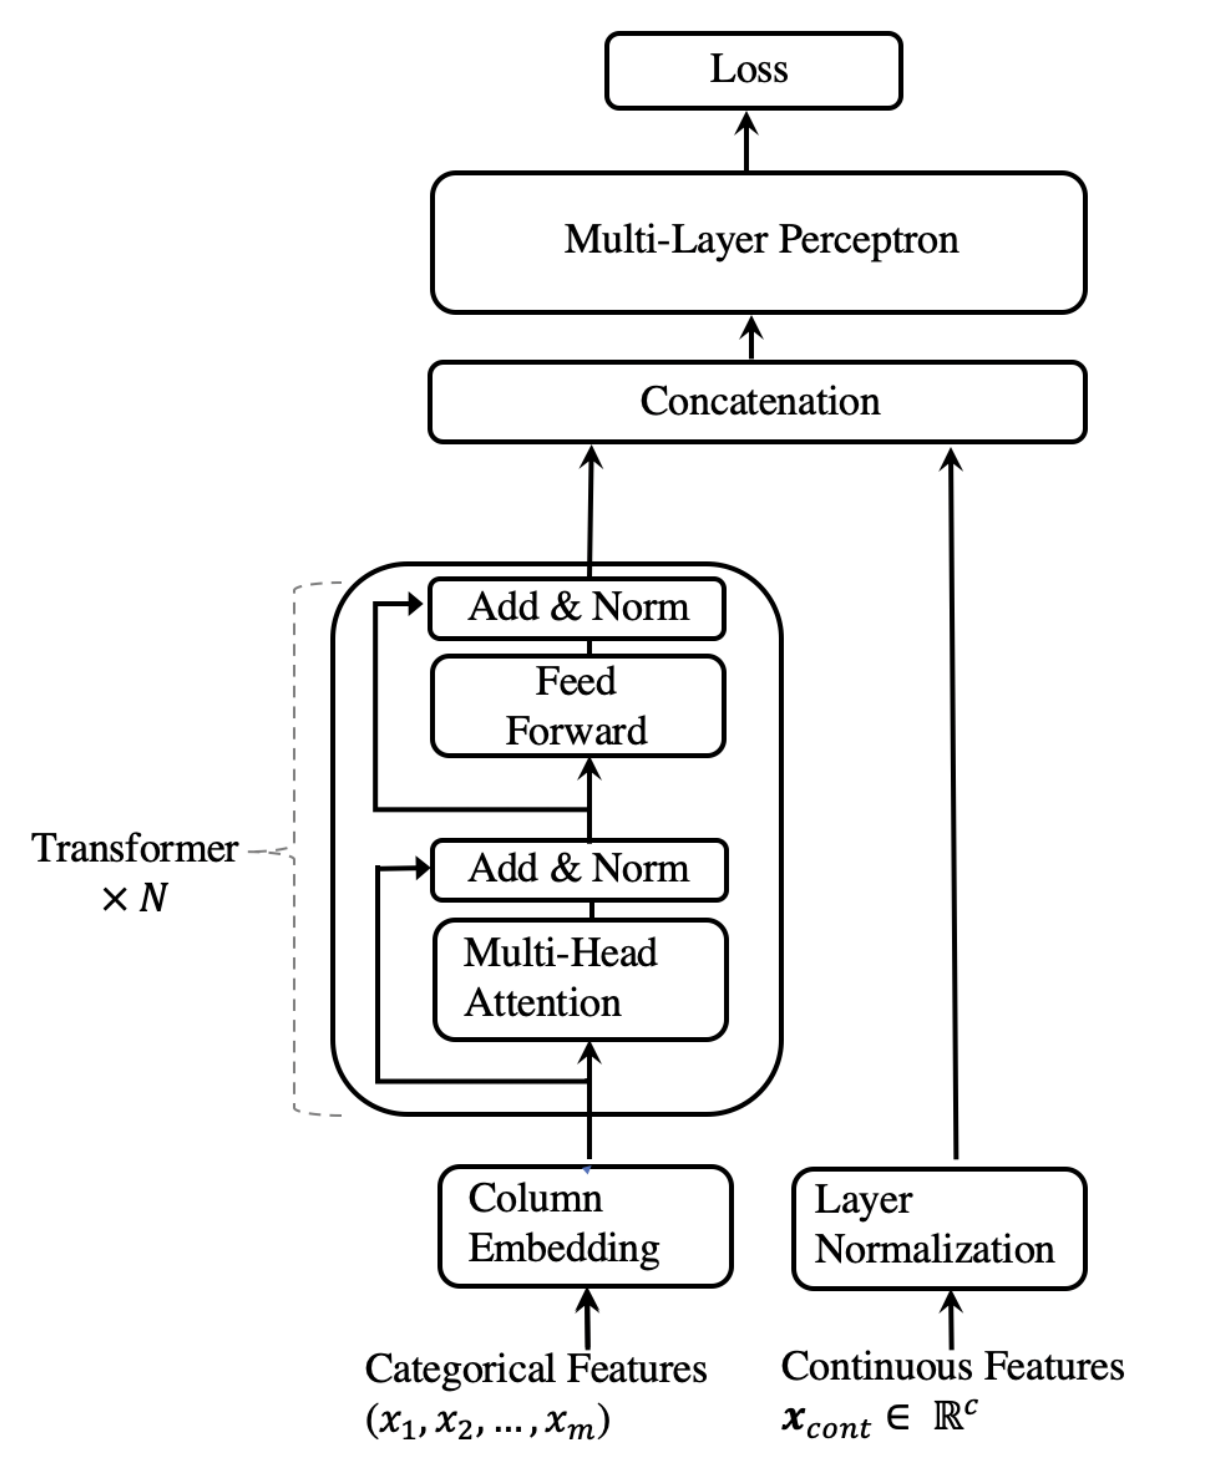
\includegraphics[width=0.4\textwidth]{images/TabTransformer.png}
    \caption{Архитектура TabTransformer}
    \label{fig:test}
\end{wrapfigure}

\noindent Учитывая впечатляющие успехи трансформерной архитектуры описанные выше, закономерно встал вопрос о применении ее для работы с табличными данными.

 Первой значимой работой в этой сфере стала статья \textit{``TabTransformer``, Xin Huang} [24], где была предложена идея передачи категориальных фичей в трансформер через стандартные контекстные эмбединги. Далее выход трансформера (а именно \texttt{<CLS>} токен) конкатенируется с численными признаками и подается в MLP.

 Основной проблемой в архитектуре TabTransformer является не самая оптимальная обработка численных признаков. Фактически для численных признаков эта модель сопоставима обычному MLP, поэтому она давала лишь небольшой прирост метрик относительно полносвязной нейронной сети. 

 Идея данного исследования состоит в том, чтобы предложить архитектуру, которая будет более эффективно обрабатывать численные признаки.

\newpage

\subsubsection{FT-Transformer}

\begin{wrapfigure}[12]{r}{0.5\textwidth}
    
    \centering
    \vspace{-6mm}
    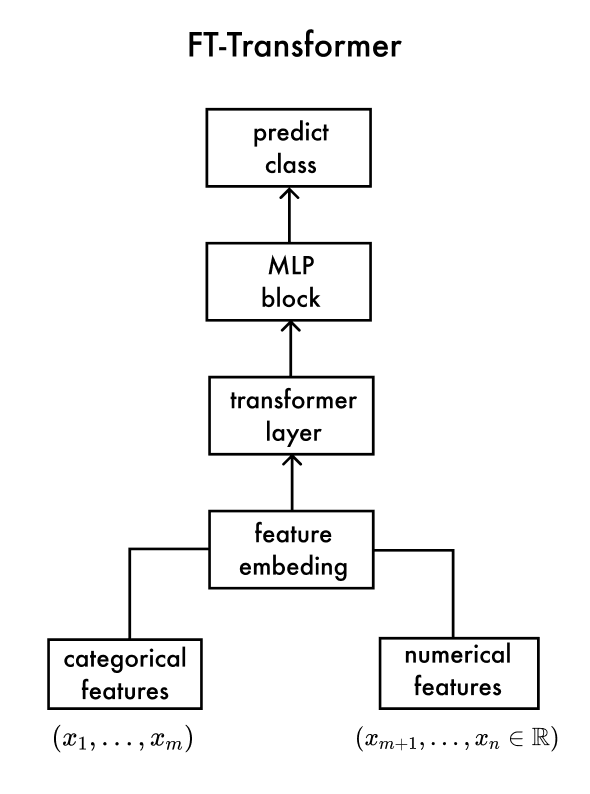
\includegraphics[width=0.43\textwidth]{images/FT_Transformer_v.png}
    \label{fig:test}
\end{wrapfigure}

\noindent Дальнейшее развитие этой идеи не заставило себя долго ждать: уже через год, исследователи из Yandex Research предложили усовершенствовать модель и подать в трансформер все признаки, а не только категориальные. Эта модель была представлена в статье \textit{``Revisiting Deep Learning Models for Tabular Data``, Gorishniy} [1] и получила название FT-Transformer (Feature Tokenizer + Transformer). Фактически, она ничем не отличается от стандартного TabTransformer, за исключением того, что численные признаки также через эмбединги подаются на вход в трансформерные слои.

В рамках данного исследования также была протестирована архитектура, построенная на базе трансформера, которая является модернизацией FT-Transformer. Как видно из схемы выше, архитектура данной нейронной сети состоит из нескольких ключевых частей:

\begin{enumerate}
    \item Энкодер - преобразует каждый признак в таблице в токен (вектор из чисел). Способ преобразования значения признака в токен отличается для категориальных и численных признаков (это обсудим позже, в пункте про эмбединги):
    \vspace{-11mm}
    \begin{flushleft}
        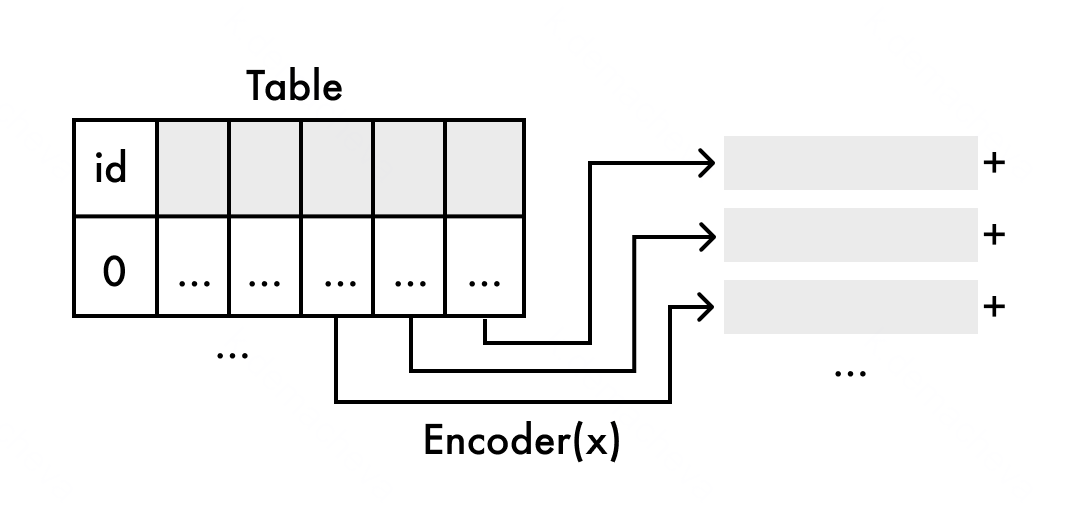
\includegraphics[width=0.8\linewidth]{images/first_segment.png}
    \end{flushleft}
    \vspace{-11mm}
    \item После предыдущего слоя формируется последовательность токенов для каждого объекта, то есть для каждой строки таблицы. Эти токены подаются в слои трансформера как последовательные данные, то есть трансформер работает с последовательностью токенов, которые в действительности являются характеристиками одного объекта:
    \vspace{-4mm}
    \begin{flushleft}
        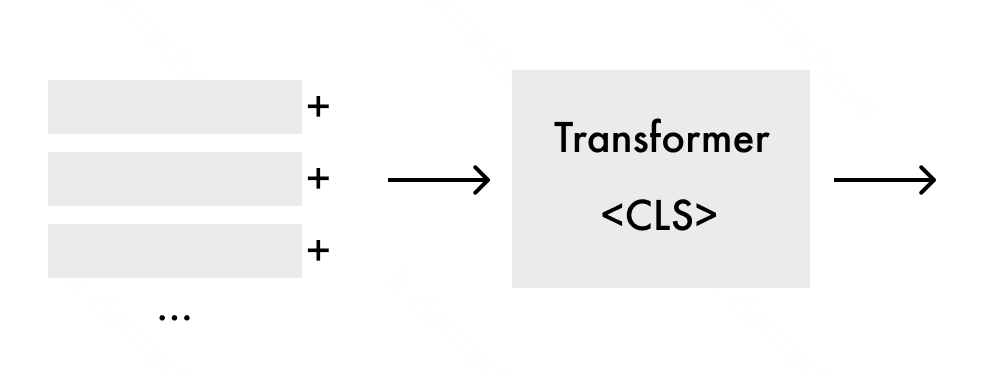
\includegraphics[width=0.8\linewidth]{images/second_segment.png}
    \end{flushleft}
    \vspace{-11mm}
    
    \item После этого используется \texttt{<CLS>} токен (специальный токен, который добавляется в начало входной последовательности и используется для агрегации информации всего входного контекста), который подается на вход в обычную полносвязную нейронную сеть и на выходе получается предсказание класса:

    \vspace{-4mm}
    \begin{flushleft}
        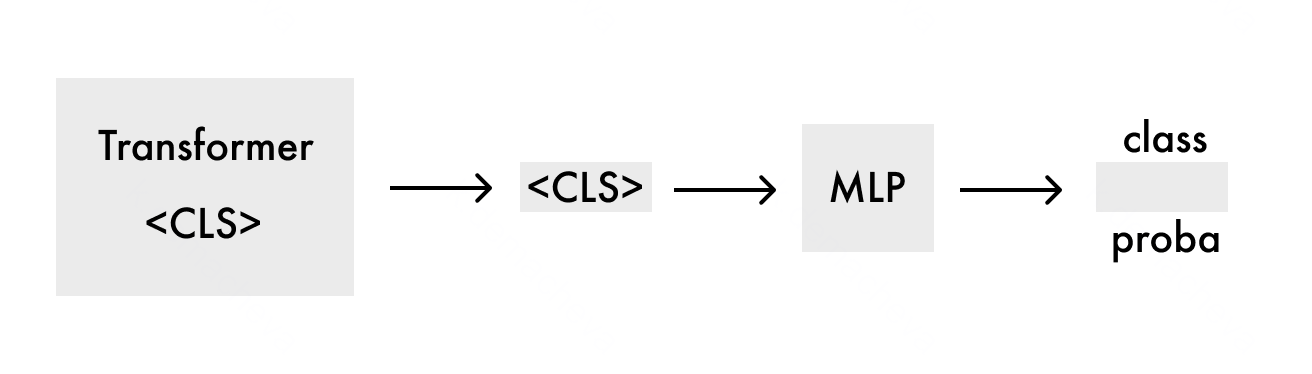
\includegraphics[width=0.8\linewidth]{images/third_segment.png}
    \end{flushleft}
    \vspace{-11mm}
\end{enumerate}

\subsubsection{MLP encoder Transformer}
\begin{wrapfigure}[12]{r}{0.5\textwidth}
    \vspace{-22mm}
    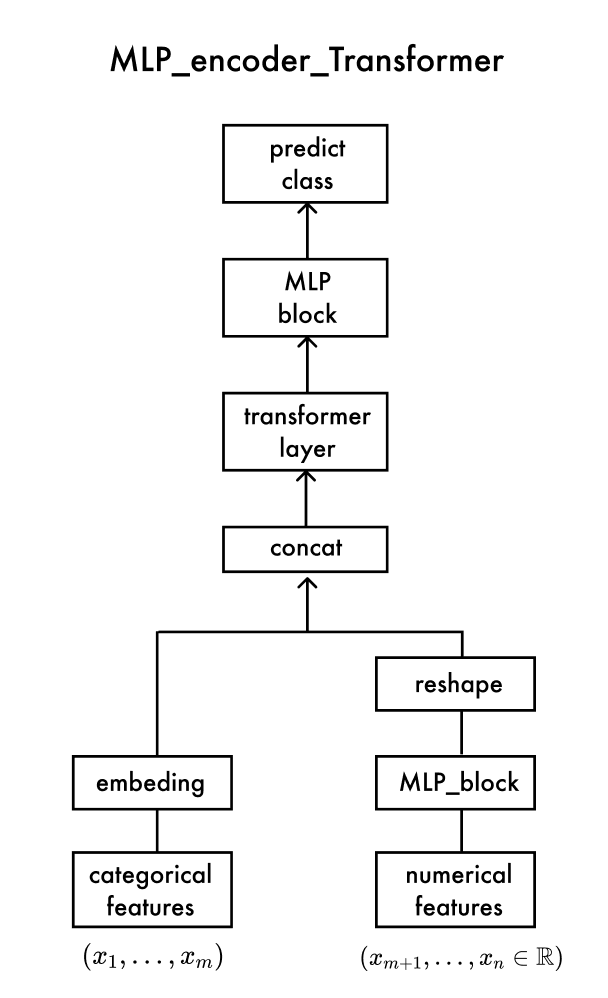
\includegraphics[width=0.43\textwidth]{images/MLP_encoder_transformer_arch.png}
    \label{fig:test}
\end{wrapfigure}

\noindent Развивая эту идею далее, можно рассмотреть еще одну интересную архитектуру. Как упоминалось ранее, основная проблема TabTransformer - неоптимальная обработка численных признаков. Модель из предыдущего пункта решала эту проблему путем перевода численных признаков в специальные токены, которые, как будет показано далее, не обучаемые и зависят только от значения конкретного признака и его распределения.

\noindent Идея \texttt{MLP encoder Transformer} -- сделать эти эмбединги обучаемыми (аналогично тому, как это работает в контекстных эмбедингах в NLP).

Рассмотрим как это будет работать: каждый численный признак подается в блок MLP для того чтобы из скалярных величин получить векторные представления - токены, размерность которых будет совпадать с размерностью эмбедингов категориальных признаков:

\begin{center}
    \vspace{-2mm}
    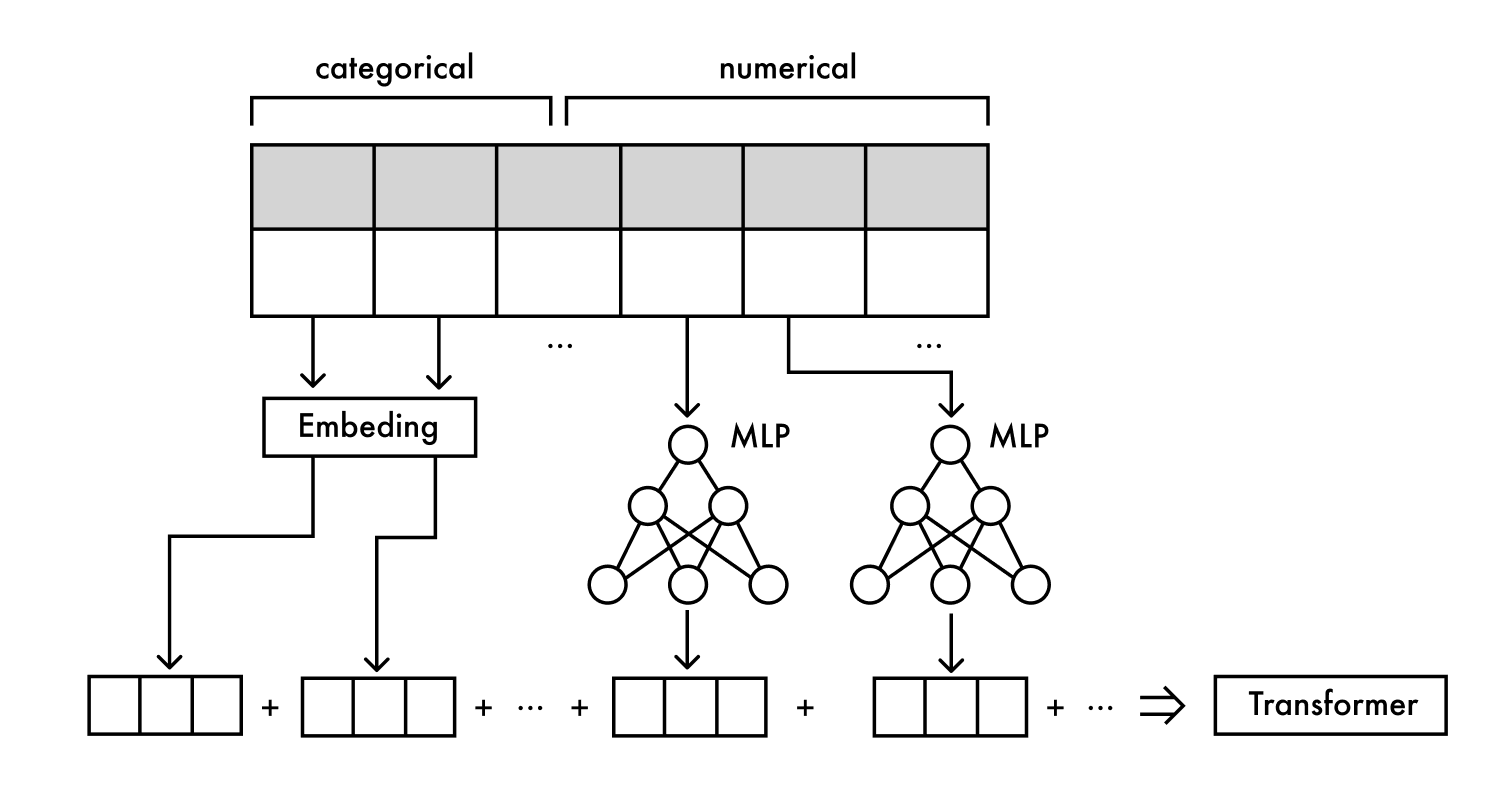
\includegraphics[width=0.8\linewidth]{images/MLP_encoder_transformer.png}
    \vspace{-3mm}
\end{center}

В остальном, приниц работы модели не меняется: полученная последовательность токенов передается в трансформерные слои, аналогично предыдущей архитектуре. На выходе получается \texttt{<CLS>} токен, который далее преобразуется в предсказание класса.

\subsection{Примеры эмбедингов}
Эмбеддинг - очень важный слой нейронной сети, позволяющий преобразовывать категориальные и численные признаки в векторные представления - токены. Эмбединг для значения признака $x_i$ вычисляется следующим образом:
\begin{equation}
T_i = f_i(x_i) \in \mathbb{R}^d \quad f_i : \mathbb{X}_i \rightarrow \mathbb{R}^d, 
\end{equation}
В современном глубоком обучении эмбеддинги играют ключевую роль в подготовке данных ко входу в модель. Недавние исследования [2] подчеркивают важность эмбеддингов в повышении эффективности трансформерных архитектур нейронных сетей. Правильный выбор эмбеддингов может существенно повлиять на качество модели, в связи с этим, в данном исследовании будет рассмотрено несколько различных типов эмбеддингов, чтобы определить их влияние на эффективность модели в задаче кредитного скоринга.

\subsubsection{Element-wise multiplication encoding}

Самый наивный вариант эмбединга, предложенный в работе о применении нейронных сетей на табличных данных от \textit{Yandex Research} [1]. Принцип вычисление $i$-го токена основан на поэлементном произведении обучаемого вектора весов $W_i$ на значение признака $x_i$. Для категориальных признаков во всех архитектурах применяется эмбединг, основанный по принципу словаря с обучаемыми весами (\texttt{CategoricalEncoder}):
\begin{align}
&T_i^{(\text{num})} = b_i^{(\text{num})} + x_i^{(\text{num})} \cdot W_i^{(\text{num})} \in \mathbb{R}^d, \\
&T_i^{(\text{cat})} = b_i^{(\text{cat})} + e_i^T W_i^{(\text{cat})} \in \mathbb{R}^d, \; \text{где } e_i^T \text{ — one-hot вектор для } x_i, \\
&T = \text{concat} \left[ T_{1^{(\text{num})}}^{(\text{num})}, \ldots, T_{k^(\text{num})}^{(\text{num})},\ T_{1^{(\text{cat})}}^{(\text{cat})}, \ldots, T_{k^{(\text{cat})}}^{(\text{cat})} \right] \in \mathbb{R}^{k \times d}.
\end{align}

\noindent Пример эмбединга для таблицы с тремя численными и двумя категориальными фичами:
\begin{center}
    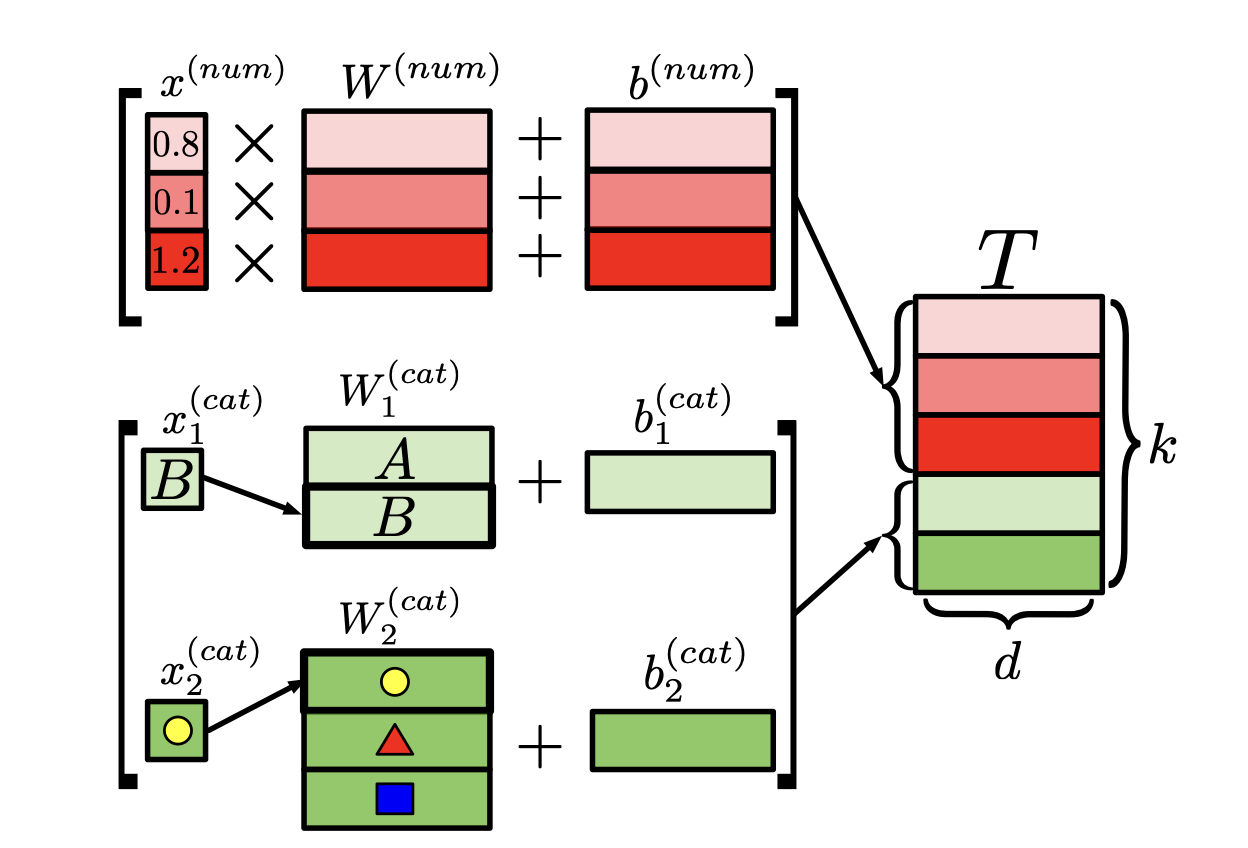
\includegraphics[width=12cm,height=7cm]{images/Default_embeding.png}
\end{center}

\subsubsection{Piecewise linear encoding}

Несколько новых эмбедингов для численных признаков на табличных данных были предложены в статье \textit{``On Embeddings for Numerical Features in Tabular Deep Learning'', Yury Gorishniy} [2]. Один из них представляет собой усовершенствованный подход бинирования (разбиение на бины).

Идея этого эмбединга очень проста и понятна: метод вдохновлен самым популярным в классическом машинном обучении кодированием - \texttt{One-Hot-Encoding}, который широко и успешно используется для представления категориальных признаков. 

Фактически, это непрерывная альтернатива \texttt{one-hot} кодированию: для $i$-го численного признака его диапазон значений разбивается на множество из $T^i$ непересекающихся интервалов $B^i_1, \ldots, B^i_T$ - бинов:

\vspace{-3mm}
\begin{align}
&\text{PLE}(x) = [e_1, \ldots, e_T] \in \mathbb{R}^T \\
&e_t = 
\begin{cases} 
0, \; x < b_{t-1} \; \text{и} \; t > 1 \\
1, \; x \geq b_t \; \text{и} \; t < T \\
\frac{x-b_{t-1}}{b_t-b_{t-1}}, \; \text{иначе} 
\end{cases}
\end{align}

\noindent Способов выбора бинов $B^i_1, \ldots, B^i_T$ может быть несколько. Вот некоторые интересные из них:

\begin{enumerate}
    \item Разделение диапазона значений в соответствии с равномерно выбранными квантилями распределения соответствующего признака на обучающей выборке:
    \begin{equation}
        b_t = Q_t \left(\left\{ x_i^{(j)} \right\}_{j \in J_{train}}\right), \text{где \(Q\) — это функция получения квантиля. }
    \end{equation}

    \item Построение решающего дерева по одному признаку в таргет. Принципиальное отличие этого подхода заключается в том, что в нем используются обучающие метки классов для построения бинов:

    \begin{tikzpicture}[
        level/.style={sibling distance=60mm/#1},
        every node/.style={circle,draw}
    ]
    \node {$x < b_2$}
        child {
            node {$x < b_1$} 
            child {
                node {$\hat{y}_1$}
                edge from parent node[left,draw=none] {yes}
            }
            child {
                node {$\hat{y}_2$}
                edge from parent node[right,draw=none] {no}
            }
            edge from parent node[left,draw=none] {yes}
        }
        child {
            node {$x < b_3$}
            child {
                node {$\hat{y}_1$}
                edge from parent node[left,draw=none] {yes}
            }
            child {
                node {$\hat{y}_2$}
                edge from parent node[right,draw=none] {no}
            }
            edge from parent node[right,draw=none] {no}
        };
    \end{tikzpicture}
    
\end{enumerate}



\subsubsection{Periodic encoding}

В последние 5 лет периодические функции стали ключевым компонентом для обработки (эмбедингов) численных входных данных. Примерами применения такого рода токенизаторов являются обработка естественного языка [9], компьютерное зрение [21], неявные нейронные представления [22]. В отличие от бинирования, данный метод сохраняет информацию о количественных различиях между признаками:
\begin{align}
f_i(x) = \text{Periodic}(x) = \texttt{concat}[\sin(v), \cos(v)] \quad \forall v = [2\pi c_1 x, \ldots, 2\pi c_k x]
\end{align}

\noindent В данной работе также исследуется эффективность применения фурье-эмбедингов.

\newpage
\section{Данные и их обработка}
\subsection{Данные}

Для экспериментов были выбраны публичные наборы данных, предоставленные крупными банками (например \textit{Home Credit Bank}, \textit{Raiffeisen}) для соревнований в области оптимизации эффективности кредитного скоринга на платформе \textbf{Kaggle}:

\begin{enumerate}
    \item \textbf{HCDR} - датасет с соревнования {Home Credit Default Risk}\footnote{https://www.kaggle.com/competitions/home-credit-default-risk}, 2018. Cодержит порядка 300 тысяч кредитных заявок клиентов с более чем 120-ю признаками из семи различных источников: выписки кредитного бюро, банковские транзакции, кредитная история, скоры внешних источников и др. Целевая переменная — факт дефолта по кредиту.

    \item \textbf{CSC} - стандартный тренировочный датасет задачи кредитного скоринга {Credit score classification}\footnote{https://www.kaggle.com/datasets/parisrohan/credit-score-classification?select=train.csv}, 2024. Он содержит порядка 50-и тысяч кредитных заявок клиентов с более чем 30-ю признаками, таргет - факт дефолта по кредиту.

    \item \textbf{ADP} - датасет с соревнования {American Express - Default Prediction}\footnote{https://www.kaggle.com/competitions/amex-default-prediction/data}, 2021. Задача соревнования - предсказать вероятность того, что клиент не погасит задолжность по его кредитной карте, в будущем, основываясь на его ежемесячном профиле. Таргет - отсутствие просрочки на протяжении 180 дней после открытия карты.
    
    
\end{enumerate}

Во всех датасетах доля таргетов порядка $4-8\%$, что сразу же указывает на сильный классовый дисбаланс

\subsection{Обработка данных}

Для обработки данных был реализован специальный класс
\texttt{PrepareTabularData}, который выполняет все этапы предварительной обработки данных для каждой из исследуемых архитектур нейронной сети - по разному. Порядок работы класса следующий:

\begin{enumerate}
    \item Загружает данные, разделяет все признаки на категориальные и численные (определение типа происходит по количеству уникальных значений), заполняет пропуски, для удобства дальнейшей обработки признаков делит датасет на три части - категориальные признаки, численные признаки и таргет.
    
    \item Разделяет данные на train : test : validate в пропорциях $1-\alpha-\beta : \alpha : \beta$. При разделении данных используется стратификация, чтобы сохранить исходное соотношение классов.
    
    \item Обрабатывает признаки:
    \begin{itemize}
        \item \textbf{Численные признаки} - нормализует (по умолчанию при помощи \texttt{StandardScaler}) и токенизирует их при помощи одного из исследуемых энкодеров (по умолчанию применяется \texttt{PiecewiseLinearEncoder}).
        
        \item \textbf{Категориальные признаки} - применяет \texttt{OneHotEncoder} в случае бустинга или \texttt{OrdinalEncoder} для нейронных сетей, чтобы потом их можно было подать в \texttt{CategoricalEncoder}.
        
    \end{itemize}
    
    \item Преобразует полученные данные в \texttt{PyTorch}-тензоры и переносит их на \texttt{GPU}, если это возможно.
\end{enumerate}

\newpage
\section{Эксперименты}
\subsection{Метрики качества модели}

В задаче кредитного скоринга, как упоминалось ранее, мы сталкиваемся со стандартной для задач классификации проблемой - сильным дисбалансом классов. Это в первую очередь связано со спецификой задачи кредитного скоринга - банку просто невыгодно выдавать кредиты людям, которые деньги не вернут, поэтому таргетов (выходов в дефолт) в выборке обычно очень мало - порядка $2-5\%$. В подобных ситуациях классическая метрика классификации - точность предсказания ($\textit{accuracy}$) становится малоинформативной, потому что даже модель предсказывающая всегда класс \texttt{0} будет иметь высокие показатели ($\textit{accuracy} = 0.98$), но, очевидно, окажется абсолютно бесполезной для выявления рисков, поэтому, для корректной оценки качества модели, будут использоваться метрики устойчивые к дисбалансу.

\subsubsection{Precision и Recall}

\noindent Для подсчета точности и полноты используются общепринятые обозначения - $TP$ (истинно положительные), $TN$(истинно отрицательные), $FP$ (ложно положительные) и $FN$ (ложно отрицательные) значения:

\begin{enumerate}
    \item $Precision = \frac{TP}{TP + FP}$ - полнота (доля верных предсказаний дефолтов)

    \item $Recall = \frac{TP}{TP + FN}$ - точность (покрытие реальных дефолтов)
\end{enumerate}

\subsubsection{ROC-AUC}

\begin{wrapfigure}[9]{r}{0.45\textwidth} 
    \vspace{-25pt}
    \centering
    \includegraphics[width=0.45\textwidth]{images/ROC_curve.png}
    \caption{ROC-кривая}
\end{wrapfigure}

\noindent ROC-AUC - устойчивая к дисбалансу метрика, оценивающая способность модели ранжировать объекты по вероятности принадлежности к конкретному классу (в нашем случае - вероятности дефолта клиента). ROC-AUC - площадь под ROC-кривой - это кривая, построенная по принципу: по оси $x$ - полнота, а по оси $y$ - точность. То есть:

$$
\text{ROC-AUC} = \int_{0}^{1} \text{TPR}(FPR) d(FPR)
$$

\noindent - обычно такой интеграл подсчитывется при помощи метода трапеций.

\noindent Полученное в эксперименте значение ROC-AUC можно проинтерпретировать так:

\begin{itemize}
    \item $1$ - идеальная модель
    \item $0.5$ - абсолютно случайное угадывание класса
    \item $0$ - идеальная модель, предсказывающая классы в точности наоборот (перепутаны таргеты)
\end{itemize}

\noindent P.S. Многие крупные банки зачастую вместо ROC-AUC используют коэффициент Джини - его отнормированную версию: $\text{GINI} = 2 \cdot \text{AUC} - 1 \in [-1, 1]$

\subsubsection{Выводы о метриках}

Перечисленные выше метрики в совокупности позволяют оценить модель с разных точек зрения: ROC-AUC характеризуют способность модели к ранжированию объектов, что на самом деле является ключевым качеством скоринговой модели, Precision и Recall показывают эффективность работы с классом дефолтов - на практике для скоринга эти метрики не используются, но зато применяются в задаче кредитного и транзакционного антифрода.

Разумеется, в реальной жизни все модели кредитного скоринга оцениваются по бизнес метрикам: например, по сумме просрочки (exposure at default), сумме выданных кредитов (GMV), NPV (Net Present Value) и так далее. 

Но, поскольку доступа к таким данным нету, валидация моделей производилась по 
техническим метрикам, о которых было сказано выше, и которые являются хорошими прокси-метриками для бизнесовых показателей.

\newpage

\subsection{Эксперименты}

Эксперименты для всех архитектур и эмбедингов проводились в облачной платформе \textit{YandexCloud} на графической карте \texttt{NVIDIA A100} или \texttt{NVIDIA V100}. Обучение каждой модели нейронной сети (кроме \texttt{MLP encoder Transformer}, которая из-за случайной инициализации эмбедингов обучается сильно дольше - порядка 60-и эпох) проводилось в течение примерно 30-и эпох, чтобы избежать переобучения, но в то же время получить хорошее качество. Использовался стандартный оптимизатор \texttt{Adam} и лосс-функция \texttt{BinaryCrossEntropy} (бинарную кросс-энтропию). Для проверки качества моделей моделей была выбрана метрика \textit{ROC-AUC}, как самая эффективная в задаче бинарной классификации с дисбалансом данных. Кроме того, эта метрика является самой популярной для кредитного скоринга в большом бизнесе.

\subsubsection{Структура репозитория}

Все предложенные выше модели были реализованы на языке \texttt{Python} с использованием библиотеки \texttt{PyTorch}, исходный код лежит в репозитории GitVerse\footnote{\href{https://gitverse.ru/tsarevivan/Tabular_neural_networks/content/master}{Tabular\_neural\_networks}}. Весь код лежит в папке \texttt{experiments/src/}, структура которой устроена следующим образом:

\begin{itemize}
    \item \texttt{num\_encoders/} - все реализованные энкодеры для численных признаков
    
    \item \texttt{cat\_encoders/} - энкодер для категориальных признаков

    \item \texttt{nn\_models/} - классы всех предложенных архитектур нейронных сетей

    \item \texttt{trainer} - класс для обучения любой из предложенных моделей

    \item \texttt{prepare\_dataset} - класс для обработки датасета и подготовки его для подачи в модель
\end{itemize}

\subsubsection{Сравнение бейзлайнов моделей}

\noindent Прежде всего, посмотрим на эффективность описанных во второй главе моделей нейронных сетей (\texttt{MLP}, \texttt{ResNet} и \texttt{FT-Transformer}) без применения специфичных эмбедингов, то есть при подаче данные напрямую в модель. Полученные результаты сравнивались с одной из самых популярных и эффективных реализаций градиентного бустинга из библиотеки \texttt{CatBoost}.

\begingroup
  \renewcommand{\arraystretch}{0.8}
  \setlength{\tabcolsep}{6pt}
  \begin{table}[h]
    \caption{$\mathrm{ROC\text{-}AUC}$ на валидационном датасете} \\
    \vspace{6mm}
    \centering
    \begin{tabular}{@{}llll@{}}
      \hline
      Model         & HCDR    & ADP     & CSC      \\
      \hline
      MLP           & 0.738   & 0.731   & 0.925    \\
      ResNet        & 0.723   & 0.703   & 0.915    \\
      FT-Transformer& 0.748   & 0.742   & 0.926    \\
      CatBoost      & \textbf{0.761}\,\textcolor{OliveGreen}{$\nearrow$}
                    & \textbf{0.750}\,\textcolor{OliveGreen}{$\nearrow$}
                    & \textbf{0.939}\,\textcolor{OliveGreen}{$\nearrow$} \\
      \hline
    \end{tabular}
  \end{table}
\endgroup

Результаты в таблице 1 демонстрируют уверенное преимущество градиентного бустинга на всех датасетах, причем с большим отрывом в $\sim$1\, процентный пункт. Следовательно простое применение стандартных архитектур не позволяет получить результаты сопоставимые с бустингом - нужно модернизировать архитектуры для работы с табличными данными.


\subsubsection{Влияние эмбедингов численных признаков на качество модели}

\noindent Далее, с целью улучшения качества моделей были исследованы различные виды токенизации численных признаков. На примере базовой архитектуры MLP были протестированы три типа эмбеддингов и вариант без какой-либо специальной обработки:

\begin{itemize}
    \item WithoutEncoder -- без необычного кодирования: численные признаки подаются в исходном виде
    \item PeriodicEncoder -- фурье-кодирование, преобразующее численные  признаки в пространство синусов и косинусов
    \item PiecewiseLinearEncoder -- кусочно-линейное преобразование
    \item ElementWiseMultiplEncoder -- поэлементное умножение на матрицу весов
\end{itemize}

\noindent В данной архитектуре эмбединги применяются так: каждый признак после прохождения слоя эмбединга разворачивается в токен (вектор чисел), после этого все полученные векторы конкатенируются и подаются на вход полносвязного слоя. Как можно заметить, размерность входа в MLP в таком случае увеличивается в \texttt{embeding\_size} раз, значит сильно растет и количество обучаемых параметров. Архитектура в данном случае выглядит так:

\begin{center}
    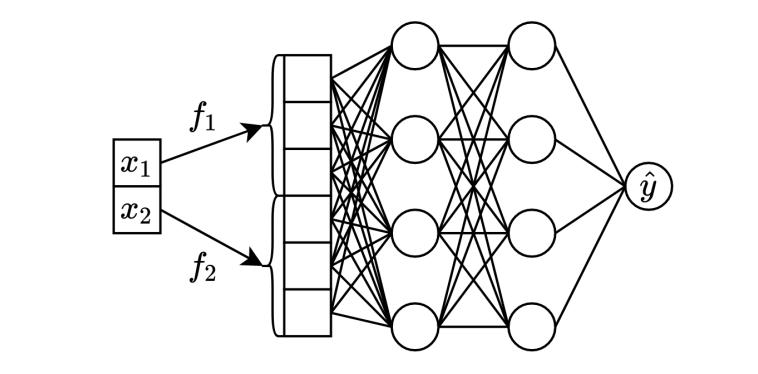
\includegraphics[width=0.7\linewidth]{images/MLP_embeding.jpeg}
\end{center}
\vspace{-6mm}
\noindent В результате эксперимента, были получены такие результаты:

\begin{table}[h]
\centering
\caption{Влияние различных энкодеров на качество MLP модели}
\vspace{10pt} 
\begin{tabular}{lccc}
\hline
Энкодер & HCDR & ADP & CSC \\
\hline
Without Encoder & 0.738 & 0.744 & 0.931 \\
PeriodicEncoder & 0.712 & 0.683 & \textbf{0.932} \textcolor{OliveGreen}{$\nearrow$} \\
PiecewiseLinearEncoder & \textbf{0.752} \textcolor{OliveGreen}{$\nearrow$} & \textbf{0.753} \textcolor{OliveGreen}{$\nearrow$} & 0.917 \\
ElementWiseMultiplEncoder & 0.72 & 0.712 & 0.896 \\
\hline
\end{tabular}
\end{table}

В среднем наилучшие результаты показывает кусочно-линейное кодирование, поэтому в итоговом эксперименте для сравнения моделей оно будет использоваться как основное для всех архитектур.

\subsubsection{Финальный эксперимент}

В финальном эксперименте были рассмотрены бейзлайновые модели - \texttt{MLP}, \texttt{ResNet} с применением кусочно-линейного эмбединга и модели основанные на механизме внимания - \texttt{PLE-encoder Transformer} (также вариант с PLE-кодированием), \texttt{MLP-encoder Transformer} (обучаемые эмбединги численных признаков). Полученные результаты (смотреть таблицу 3)  демонстрируют высокую конкурентоспособность нейронных сетей, основанных на идее трансформера и адаптированных под табличные данные. Да, возможно, на данный момент бустинг все же остается предпочтительным способом из-за своей простоты и эффективности, но потенциал развития трансформеров в задаче кредитного скоринга - огромен.

\begin{table}[h]
    \centering
    \caption{$\textit{ROC-AUC}$ на валидационном датасете}
    \vspace{2pt}

    \begin{tabular}{llll}
        \hline
        Model & HCDR & ADP & CSC \\
        \hline
        PLE-encoder MLP & 0.753 & 0.745 & 0.925 \\
        PLE-encoder ResNet & 0.727 & 0.729 & 0.920 \\
        PLE-encoder Transformer & 0.758 & \textbf{0.756} \textcolor{OliveGreen}{$\nearrow$} & \textbf{0.943} \textcolor{OliveGreen}{$\nearrow$} \\
        MLP-encoder Transformer & 0.733 & 0.743 & 0.928 \\
        CatBoost & \textbf{0.761} \textcolor{OliveGreen}{$\nearrow$} & 0.750 & 0.939 \\
        \hline
    \end{tabular} 
    \label{tab:plain}
\end{table}

Также хотелось бы отметить, что использование механизма внимания дает значительный прирост качества по сравнению с бейзлайновыми архитектурами \texttt{MLP}, \texttt{ResNet}, за счет чего трансформерные модели стабильно превосходят их на всех трех датасетах. 

Кроме того, архитектура \texttt{MLP-encoder Transformer} обучается гораздо дольше остальных из-за случайной стартовой инициализации эмбедингов. Здесь возможно дальнейшее развитие идеи: например, можно инициализировать эмбединги кусочно-линейным способом, а потом тюнить их в процессе обучения. Такой подход может привести к росту эффективности модели.

\newpage 
\section{Заключение}
В ходе данной работы были предложены несколько архитектур нейронных сетей, основанных на механизме внимания, а именно - различных адаптаций модели трансформера. Ключевой особенностью данных архитектур является внедрение в них специальных методов векторизации численных признаков (эмбедингов), поскольку первоначальные эксперименты проведенные с бейзлайнами моделей не привели к успеху.

Исследование влияния типа эмбедингов численных признаков выявило, что подбор правильной токенизации является критически важным для качества моделей. В частности, кусочно-линейное кодирование (\texttt{PLE Encoder}) в среднем показало наилучший прирост метрик.

Все модели сравнивались на нескольких публичных датасетах с классическим градиентным бустингом, а именно с одной из самых популярных его реализаций -- \texttt{CatBoost}-ом.

Финальные эксперименты показали, что предложенные трансформерные модели с применением эффективных эмбедингов вполне могут конкурировать с градиентным бустингом и показывать сопоставимые по качеству результаты, а иногда даже превосходить его по эффективности.

Таким образом, данное исследование опровергает распространенный тезис об абсолютном доминировании бустинга в задаче кредитного скоринга. Оно наглядно демонстрирует огромный потенциал нейронных сетей, ведь при грамотном проектировании и настройке трансформеры уже сейчас являются высокоэффективной альтернативой этому методу.

Кроме того, стоит отметить, что потенциал предложенных идей не до конца исчерпан. Например, в ходе работы было уделено мало времени оптимизации гиперпараметров, что открывает возможности для дальнейших исследований. Особенно интересной идеей является инициализация энкодера в модели \texttt{MLP encoder Transformer} не случайным вектором, а, например, весами предварительно настроенного кусочно-линейного энкодера.


\newpage

\section*{Список литературы}
\addcontentsline{toc}{section}{Список литературы}

\begin{enumerate}

    \item Yury Gorishniy, Ivan Rubachev, Valentin Khrulkov, Artem Babenko - Revisiting Deep Learning Models for Tabular Data, arXiv, 2106.11959, 2022
    
    \item Yury Gorishniy, Ivan Rubachev, Artem Babenko - On Embeddings for Numerical Features in Tabular Deep Learning, arXiv, 2203.05556v4, 2023
    
    \item Noam Shazeer - GLU Variants Improve Transformer, arXiv, 2002.05202, 2020
    
    \item P Aditya Sreekar, Sahil Verma, Varun Madhavan, Abhishek Persad - Unveiling the Power of Self-Attention for Shipping Cost Prediction: The Rate Card Transformer, arXiv, 2311.11694, 2023
    
    \item Yury Gorishniy, Akim Kotelnikov, Artem Babenko -
    TABM: Advancing Tabular Deep Learning With Parameter-efficient Ensembling, arXiv, 2410.24210, 2024
    
    \item Vadim Borisov, Tobias Leemann, Kathrin Seßler, Johannes Haug, Martin Pawelczyk and Gjergji Kasneci - Deep Neural Networks and Tabular Data: A Survey, arXiv, 2110.01889, 2024
    
    \item Наим Сиддики - Скоринговые карты для оценки кредитного риска, 
    
    \item Günter Klambauer, Thomas Unterthiner, Andreas Mayr - Self-Normalizing Neural Networks, arXiv, 1706.02515, 2017
    
    \item Ashish Vaswani, Noam Shazeer, Niki Parmar, Jakob Uszkoreit, Llion Jones, Aidan N. Gomez, Łukasz Kaiser, Illia Polosukhin - Attention Is All You Need, arXiv, 1706.03762, 2017
    
    \item Kaiming He, Xiangyu Zhang, Shaoqing Ren, Jian Sun - Deep Residual Learning for Image Recognition, arXiv, 1512.03385, 2015

    \item Irwan Bello, William Fedus, Xianzhi Du, Ekin D. Cubuk, Aravind Srinivas, Tsung-Yi Lin, Jonathon Shlens, Barret Zoph - Revisiting ResNets: Improved Training and Scaling Strategies, arXiv, 2103.07579, 2021

    \item Ira Shavitt, Eran Segal - Regularization Learning Networks: Deep Learning for Tabular Datasets, arXiv, 1805.06440, 2018

    \item Sercan O.Arık, TomasPfister - TabNet: Attentive Interpretable Tabular Learning,  arXiv, 1908.07442, 2019 (Tab Net)

    \item Sarkhan Badirli, Xuanqing Liu, Zhengming Xing, Avradeep Bhowmik, Khoa Doan, Sathiya S. Keerthi - Gradient Boosting Neural Networks: GrowNet, arXiv, 2002.07971, 2020 (Бустинг Нейросеток)

    \item Sergei Popov, Stanislav Morozov, Artem Babenko - Neural Oblivious Decision Ensembles for deep learning on tabular data, arXiv, 1909.06312, 2019 (Имитация деревьев нейросетями)

    \item Gowthami Somepalli, Avi Schwarzschild, Micah Goldblum, C. Bayan Bruss, C. Bayan Bruss, Tom Goldstein - SAINT: Improved Neural Networks for Tabular Data via Row Attention and Contrastive Pre-Training, arXiv, 2106.01342, 2021 (Трансформеры на табличных данных)

    \item S. Sun, M. Iyyer - Revisiting simple neural probabilistic language models, arXiv, 2104.03474v1, 2021

    \item Qiming Zhang, Jing Zhang, Yufei Xu, Dacheng Tao - Vision Transformer with Quadrangle Attention, arXiv, 2303.15105, 2023

    \item Alec Radford, Karthik Narasimhan, Tim Salimans, Ilya Sutskever - Improving Language Understanding by Generative Pre-Training, 2018

    \item Jacob Devlin, Ming-Wei Chang, Kenton Lee, Kristina Toutanova - BERT: Pre-training of Deep Bidirectional Transformers for Language Understanding, arXiv, 1810.04805, 2018

    \item Y. Li, S. Si, G. Li, C. Hsieh, and S. Bengio - Learnable fourier features for multi-dimensional spatial positional encoding, arXiv, 2106.02795, NeurIPS, 2021

    \item B. Mildenhall, P. P. Srinivasan, M. Tancik, J. T. Barron, R. Ramamoorthi, R. Ng. Nerf - Representing scenes as neural radiance fields for view synthesis, arxiv, 2003.08934, ECCV, 2020

    \item Gowthami Somepalli, Micah Goldblum, Avi Schwarzschild, C. Bayan Bruss, Tom Goldstein - SAINT: Improved Neural Networks for Tabular Data via Row Attention and Contrastive Pre-Training, 2106.01342, 2021

    \item Xin Huang, Ashish Khetan, Milan Cvitkovic, Zohar Karnin - TabTransformer: Tabular Data Modeling Using Contextual Embeddings, arXiv, 2012.06678v1, 2020

    \item Scott M. Lundberg, Su-In Lee - A Unified Approach to Interpreting Model Predictions (SHAP), arXiv, 1705.07874, 2017

\end{enumerate}

\end{document}

